
\subsection{Prezentacja Wirtingera}
\index{prezentacja!Wirtingera|(}%
Perko \cite{perko2016} pisze, że na wykładzie w 1905 roku (którego nigdy nie spisano) ,,Wirtinger otworzył drzwi do barwnego świata przestrzeni nakryciowych''\footnote{\emph{,,I think covering spaces can be understood by fifth graders''} -- Kenneth Perko tamże}, rozkładając dopełnienie węzła na komórki, co doprowadziło do prezentacji grupy podstawowej.
\index[persons]{Wirtinger, Wilhelm}%
\index[persons]{Perko, Kenneth}%
Jest to skończona prezentacja, w~której wszystkie relacje są postaci $w g_i w^{-1} = g_j$, gdzie $w$ to pewne słowo na generatorach $g_1, \ldots, g_k$.
% In a 1905 lecture that he never wrote down, Wirtinger opened the door to a colorful world of covering spaces. His cellular decomposition of a knot's complement in 3-space furnished an algorithm for presenting its fundamental group. - Perko, "Historical highlights of non-cyclic knot theory"
Pokażemy zarys konstruktywnego algorytmu, który w wygodny sposób zamienia skrzyżowania diagramu w relacje.

\begin{proposition}
    Grupa każdego zorientowanego węzła posiada prezentację Wirtingera.
\end{proposition}

\begin{proof}
    Niech $K$ będzie zorientowanym węzłem.
    Wybierzmy dowolny diagram, początkowy punkt na tym diagramie i przemierzajmy węzeł, nazywając kolejne włókna $x_1, x_2, \ldots x_{n}$.
    To będą generatory grupy.
    Do każdego skrzyżowania przypisujemy relację zgodnie z poniższymi regułami, w zależności od znaku skrzyżowania:
\begin{comment}
    \begin{figure}[H]
        \begin{minipage}[b]{.48\linewidth}
            \[
                \HugeWirtingerPlus
            \]
            \subcaption{skrzyżowanie dodatnie: $x_j = x_k x_{j+1} x_k^{-1}$}
        \end{minipage}
        \begin{minipage}[b]{.48\linewidth}
            \[
                \HugeWirtingerMinus
            \]
            \subcaption{skrzyżowanie ujemne: $x_j = x_k^{-1} x_{j+1} x_k$}
        \end{minipage}
    \end{figure}
\end{comment}
\noindent
    Oto mnemotechnika ułatwiająca zapamiętywnaie relacji.
    Wyobraźmy sobie zorientowaną przeciwnie do ruchu wskazówek zegara ścieżkę wokół skrzyżowania.
    Poruszamy się po niej i kiedy mijamy włókno biegnące do skrzyżowania, zapisujemy jego symbol, a kiedy włókno biegnie od skrzyżowania na zewnątrz, zapisujemy odwrotność jego symbolu.
    Tak uzyskane czteroliterowe słowo jest równe $1$ w grupie węzła.
\end{proof}

Porządny dowód znaleźliśmy w podręczniku Stillwella \cite[s. 144-147]{stillwell1993}: używa twierdzenia Seiferta-van Kampena.
Nie będziemy go przepisywać, ograniczymy się tylko do pożyczenia dwóch obrazków:

\begin{figure}[H]
    \centering
\begin{comment}
    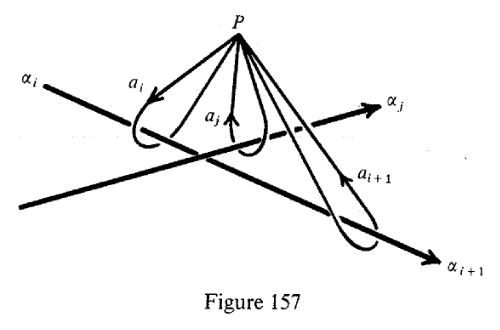
\includegraphics[height=0.28\linewidth]{../data/stillwell-157.png}
    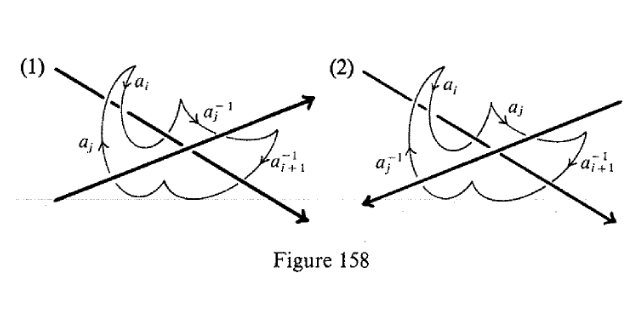
\includegraphics[height=0.28\linewidth]{../data/stillwell-158.png}
\end{comment}
    \caption[caption-stillwell]{Kontrakcja krzywych do punktu}
\end{figure}

\begin{corollary}
    Niech $G$ będzie grupą węzła.
    Wtedy jej abelianizacja jest nieskończoną grupą cykliczną: $G^{\operatorname{ab}} \cong \Z$.
\end{corollary}

Jedna z relacji w prezentacji Wirtingera jest zbędna -- wynika z pozostałych.
Fakt ten zazwyczaj podaje się bez dowodu, dlatego warto wspomnieć, że nie zapomniał o nim Rolfsen \cite[s. 56-60]{rolfsen1976}, za co serdecznie mu dziękujemy.

\begin{proof}
    Relacja $a_ia_ja_i^{-1}a_k^{-1}=1$ po przejściu do abelianizacji przyjmuje postać $a_j = a_k$.
    Oznacza to, że etykieta łuku nie zmienia się podczas przejścia pod każdym skrzyżowaniem, zatem wszystkie etykiety są takie same.

    Można też zauważyć, że abelianizacją grupy podstawowej węzła jest pierwsza grupa homologii okręgu, czyli $\Z$.
\end{proof}

Michel Kervaire \cite{kervaire1965} pokazał, jakie własności musi posiadać grupa węzła (i~wiemy o~tym, bo przeczytaliśmy książkę Kawauchiego \cite[tw. 14.1.1]{kawauchi1996}):
\index[persons]{Kervaire, Michel}%

\begin{proposition}
\index{południk}%
\index{homologia!druga grupa homologii}%
    Niech $G$ będzie grupą węzła $S^n \subseteq S^{n+2}$.
    Wtedy:
    \begin{enumerate}
        \item grupa $G$ jest skończenie prezentowana,
        \item abelianizacja $G/G'$ jest nieskończoną grupą cykliczną,
        \item druga grupa homologii $H_2(G) = 0$ jest trywialna,
        \item istnieje element $x \in G$ zwany południkiem taki, że $G$ jest najmniejszą podgrupą normalną $G$, która zawiera $x$.
        \index{południk}%
    \end{enumerate}
\end{proposition}

Wyżej wymienione warunki konieczne są także wystarczające, jeżeli $n \ge 3$, jednakże problem pełnej charakteryzacji w~czwartym wymiarze jest otwarty.
Warunki 2. i 3. wynikają z~dualności\footnote{Niech $X$ będzie zwartą, lokalnie ściągalną podprzestrzenią sfery $S^n$. Wtedy $\tilde {H}_{q}(S^n \setminus X) \cong \tilde H^{n-q-1}(X)$. Założenie o~lokalnej ściągalności można pominąć, jeśli pracuje się z kohomologią Čecha.\index{kohomologia!Čecha}} Alexandera, zaś 1. i 4. stanowią przeformułowanie prezentacji Wirtingera.

\index{prezentacja!Wirtingera|)}%
% koniec podsekcji Prezentacja Wirtingera

